\section{METODOLOGI}

% Ubah bagian-bagian berikut dengan isi dari pendahuluan

\subsection{Data dan Peralatan/ Data dan Alat Bantu/ Material }
\label{sec:datadanperalatan}

\textbf{Hardware}
\begin{enumerate}[label=(\alph*)]
   \item ESP32
% Contoh input gambar
\begin{figure}[ht]
  \centering

  % Ubah dengan nama file gambar dan ukuran yang akan digunakan
  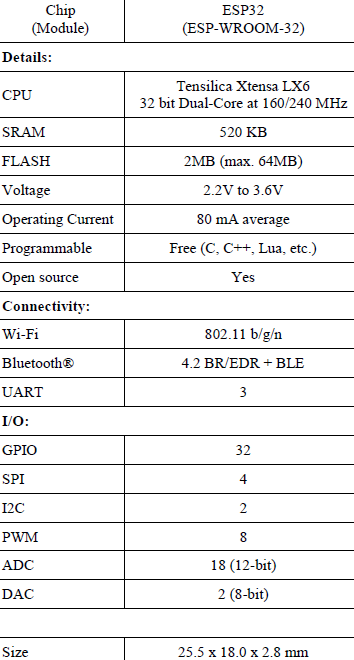
\includegraphics[scale=0.5]{gambar/tabelsatuu.png}

  % Ubah dengan keterangan gambar yang diinginkan
  \caption{Spesifikasi ESP32 }%\citep{roketluarangkasa}.}
  \label{fig:tabelsatu}
\end{figure}
	\item Relay Pompa
	\begin{itemize}
		\item Tipe : MK2P-1
		\item Volt : 220 V AC 10 A
	\end{itemize}
	\item DS18B20 Digital Temperature Sensor
	\begin{itemize}
		\item Operating voltage: 3.0~ 5.5V
		\item ±0.5°C Akurasi dari -10°C ke +85°C
		\item Usable temperature range: -55 to 125°C (-67°F to +257°F)
		\item Query time kurang dari 750ms
		\item Diameter Kabel: 4mm(0.16")
		\item Panjang: 90cm(35.43")
	\end{itemize}
	\item pH Meter Sensor dengan Modul PH-4502C (Analog)
	\begin{itemize}
		\item Heating voltage : 5 ± 0.2V (AC · DC)
		\item Working current : 5-10mA
		\item Range konsentrasi yang dapat dideteksi : PH 0-14
		\item Range deteksi suhu : 0-80 °
		\item Waktu respon :  $\leq 5S$
		\item Settling Time : $\leq 60S$
		\item Daya Komponen : $\leq 0.5W$
		\item Ukuran Modul: 42mm × 32mm × 20mm
		\item Output: analog voltage signal output
	\end{itemize}
	\item Converter Tegangan \\
	AC-DC Konverter Adaptor
	\begin{itemize}
		\item	Input AC : 220V +/- 15 \%
		\item	Output DC : 12V ~ 2A
		\item	Berat : 200gr
		\item	Tipe Connector 5,5mm
		\item	Panjang Kabel 100cm
	\end{itemize}
\vspace{0.5cm}
	DC-DC Step-Down Konverter
	\begin{itemize}
	\item Voltase Input : 4.75V-23V
	\item Voltase Output: 1.0V-17V
	\item Arus Output : menurunkan nilai 3A, panjang 1.8A
	\item Efisiensi Konversi : 96\% (maksimum)
	\item Frekuensi Switching : 340KHz
	\item Load regulation: ±0.5 \%
	\item Voltage regulation: ±2.5 \%
	\item Dimensi Eksternal: 17 * 11 * 3.8 (P * L * T) (mm
	\end{itemize}
	\item Converter ADC eksternal (ADS1115)
	\begin{itemize}
	\item Resolusi: 16 Bits
	\item Programmable Sample Rate: 8 to 860 Samples/Detik
	\item Power Supply : 2.0V to 5.5V
	\end{itemize}
	\item Laptop dengan spesifikasi :
	\begin{itemize}
	\item Prosesor AMD Ryzen 5 5500U dengan Radeon Graphics (12CPUs), ~2.1GHz
	\item Memory RAM 8192 MB
	\end{itemize}
	Penggunaan Laptop adalah untuk pemrograman mikrokontroller, website, dan pembuatan model prototipe tambak (akuarium kustom)
	\item Pompa Submersibel Akuarium (2 buah)
	\begin{itemize}
	\item Tegangan : 220-240V
	\item Daya : 5 Watt
	\item HMax : 90Cm
	\item Output : 380L/Jam
	\item Diameter Outlet : 1/2 inch
	\end{itemize}
\end{enumerate}

\textbf{Software}
\begin{itemize}
	\item Arduino IDE
	\item Visual Studio Code
	\item AutoCad Fusion360
\end{itemize}

\textbf{Material}
\begin{itemize}
	\item Kaca untuk Prototipe Tambak berupa Akuarium Kustom (100 cm x 100 cm x 30 cm)
	\item Selang standard akuarium (ukuran sekitar 5/6 in)
\end{itemize}

\subsection {Metodologi Penelitian}
\label{sec:metodologipenelitian}


% Contoh input gambar
\begin{figure}[htbp]
  \centering

  % Ubah dengan nama file gambar dan ukuran yang akan digunakan
  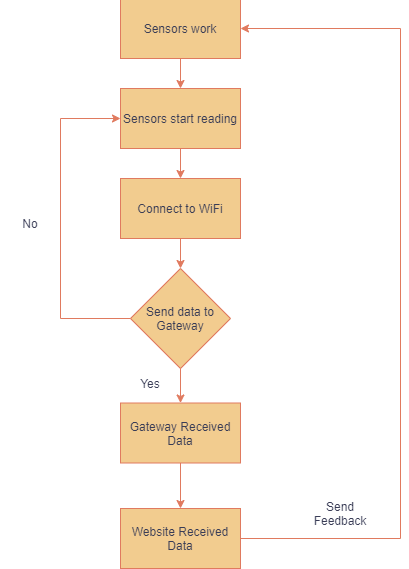
\includegraphics[scale=0.5]{gambar/diagramsatuu.png}

  % Ubah dengan keterangan gambar yang diinginkan
  \caption{Blok Diagram Metodologi Sistem} %  \citep{roketluarangkasa}.}
  \label{fig:diagramsatu}
\end{figure}

% Contoh input gambar
\begin{figure}[htbp]
  \centering

  % Ubah dengan nama file gambar dan ukuran yang akan digunakan
  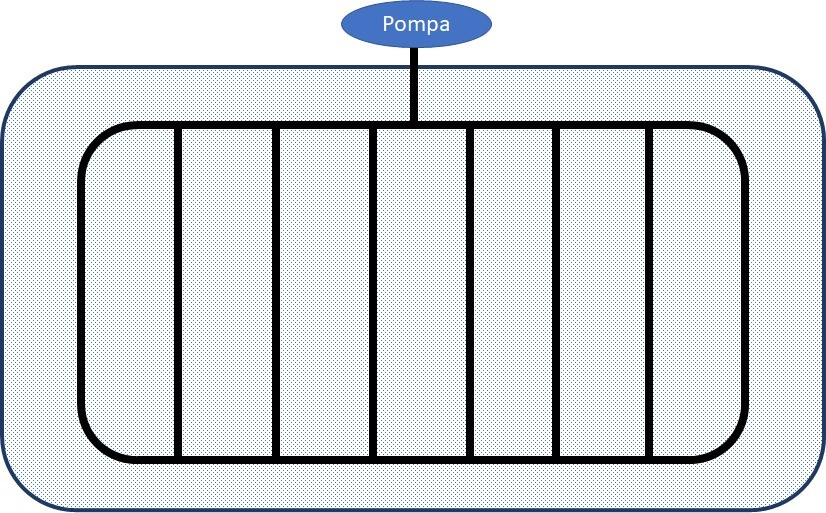
\includegraphics[scale=0.4]{gambar/bentukpipa.jpg}

  % Ubah dengan keterangan gambar yang diinginkan
  \caption{Bentuk Pipa sipon yang digunakan untuk menggantikan pekerjaan petambak}%  \citep{roketluarangkasa}.}
  \label{fig:bentukpipa}
\end{figure}

% Contoh input gambar
\begin{figure}[htbp]
  \centering

  % Ubah dengan nama file gambar dan ukuran yang akan digunakan
  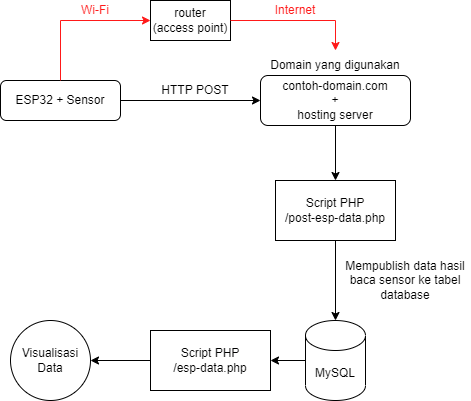
\includegraphics[scale=0.7]{gambar/metodekomunikasi.png}

  % Ubah dengan keterangan gambar yang diinginkan
  \caption{Metode Komunikasi dari Microcontroller ke Web}%  \citep{roketluarangkasa}.}
  \label{fig:metodekomunikasi}
\end{figure}

% Contoh input gambar
\begin{figure}[htbp]
  \centering

  % Ubah dengan nama file gambar dan ukuran yang akan digunakan
  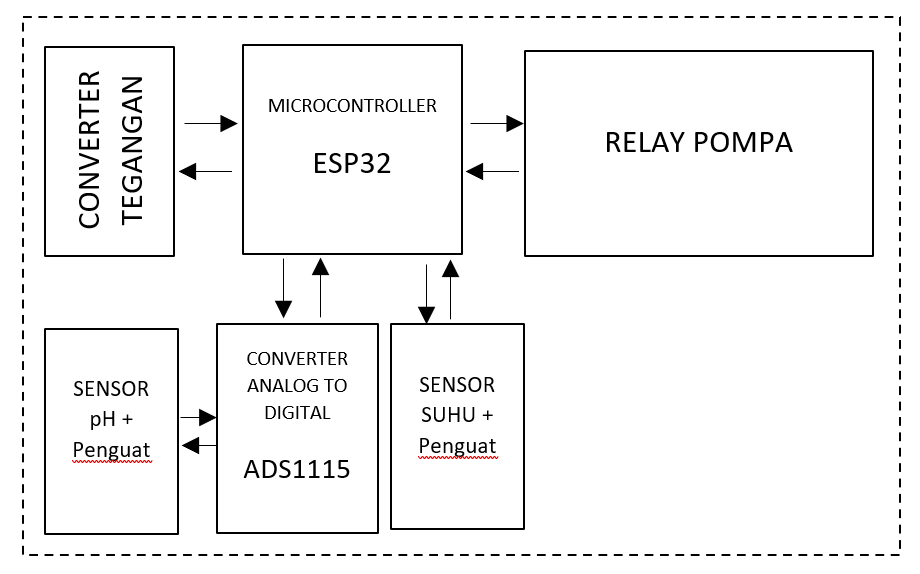
\includegraphics[scale=0.5]{gambar/blok.png}

  % Ubah dengan keterangan gambar yang diinginkan
  \caption{Blok Komponen Alat Sistem Otomasi Sipon dan Monitoring} % \citep{roketluarangkasa}.}
  \label{fig:metodekomunikasi}
\end{figure}



\begin{enumerate}
\item Cara Kerja Sistem \\
Sensor pada alat akan mengambil data yang diperlukan, yang kemudian akan diteruskan menuju Gateway dengan koneksi Wi-Fi pada modul, setelah data diterima Gateway, data akan diteruskan ke website yang mana untuk data sensor akan ditampilkan pada website tersebut. Untuk data relay, website memberikan feedback kepada relay yang nantinya akan menyebabkan relay berfungsi sesuai dengan feedback dari website.
\item Model Pipa \\
Untuk menggantikan metode umum proses sipon yang mana memerlukan petambak untuk mengitari tambaknya (Sebagian besar menggunakan pola S atau ular ), digunakan pipa yang berbentuk sesuai dengan ilustrasi diatas (gambar 2), dengan keterangan kotak biru sebagai tambak, titik biru sebagai air, kemudian garis hitam sebagai pipa (diameter sekitar 1in). Samping pipa akan diberi lubang dengan diameter 2 – 5 cm yang kemudian akan diletakkan pada dasar tambak, dengan tujuan dapat menyedot keseluruhan air dengan merata.
\item Website \\
Untuk komunikasi antara alat dengan website, menggunakan koneksi Wi-Fi yang mana sudah terpasang pada modul, kemudian menggunakan protokol MQTT untuk mengirimkan data pada domain website, lalu data akan disimpan pada database dengan menggunakan MongoDB, setelah itu dengan memanfaatkan websocket, node.js, dan vue.js, data akan divisualisasikan pada website. Sedangkan untuk komunikasi dari website menuju relay hampir identik dengan alur sebelumnya, hanya saja dimulai dari website dan  berakhir ke relay atau aktuator itu sendiri.
\item Alat Pada Sistem \\
Dalam alat yang  akan digunakan pada sistem, terdapat komponen seperti  converter tegangan, Microcontroller ESP32 dengan build-in Wi-Fi, Relay Pompa, Sensor pH dan sensor temperatur dengan modul penguatnya masing – masing,  serta konverter analog ke digital (ADS1115) untuk menghubungkan mikrokontroller dengan sensor yang masih analog.
\end{enumerate}